\chapter{Bài 2. Vấn đề an toàn trong vật lí}
\begin{center}
	\textit{(1 tiết)}
\end{center}
\section{MỤC TIÊU DẠY HỌC}
\begin{center}
	\begin{longtable}{|M{2.5cm}|L{12.5cm}|M{2cm}|}
		\hline
		\thead{Biểu hiện\\ năng lực} & \thead{Mục tiêu} & \thead{STT}\\
		\hline
		\multicolumn{3}{|c|}{\textbf{ Năng lực vật lí}}\\
		\hline
		1.1 & Thảo luận để nêu được các quy tắc an toàn trong nghiên cứu và học tập môn Vật lí & 1\\
		\hline
		\multicolumn{3}{|c|}{\textbf{Năng lực chung}}\\
		\hline
		GT - HT& Tích cực đóng góp ý kiến trong quá trình thảo luận, biết sử dụng ngôn ngữ kết hợp với các loại phương tiện phi ngôn ngữ đa dạng để trình bày các kết quả thảo luận nhóm về các quy tắc an toàn.	& 2\\
		\hline
		
	\end{longtable}
\end{center}
\section{THIẾT BỊ DẠY HỌC VÀ HỌC LIỆU}
\begin{itemize}[topsep=0pt]
	\item SGK.
	\item Phiếu học tập.
\end{itemize}
\section{TIẾN TRÌNH DẠY HỌC}
\subsection{TIẾN TRÌNH}
\begin{center}
	\begin{longtable}{|L{2.75cm}|C{1.25cm}|L{5cm}|L{3.5cm}|L{4cm}|}
		\hline
		\thead{Tiến trình} & \thead{Mục\\tiêu} & \thead{Nội dung dạy học \\trọng tâm} & \thead{PP,\\ KTDH} & \thead{Phương pháp \\đánh giá}\\
		\hline
		\textbf{Hoạt động 1:} Tìm hiểu vấn đề an toàn trong nghiên cứu và học tập vật lí& 1, 2  & Quy tắc an toàn trong nghiên cứu và học tập môn Vật lí  & PP: Dạy học hợp tác.\newline
		KTDH: Kĩ thuật "tia chớp" & GV đánh giá dựa trên kết quả báo cáo thảo luận nhóm của HS.\newline
		PP đánh giá: quan sát, nghe. \\
		\hline
		\textbf{Hoạt động 2:} Luyện tập& 1, 2  & Luyện tập các quy tắc an toàn trong nghiên cứu và học tập môn Vật lí  & PP: Đàm thoại\newline KTDH: Kĩ thuật "tia chớp"& GV đánh giá dựa trên bài tập cá nhân của HS.\newline
		PP đánh giá: quan sát, nghe. \\
		\hline
	\end{longtable}
\end{center}
\subsection{CÁC HOẠT ĐỘNG HỌC}
\hoatdong{Tìm hiểu vấn đề an toàn trong nghiên cứu và học tập vật lí}
{
HS thảo luận để nêu được các quy tắc an toàn trong nghiên cứu và học tập môn vật lí.
}
{Phiếu học tập + Phần trình bày kết quả thảo luận của nhóm HS.

}
{\textit{\underline{* GV chuyển giao nhiệm vụ học tập}}\\
	GV chia lớp thành 4 nhóm. GV yêu cầu các nhóm HS đọc kĩ SGK và thực hiện 2 nhiệm vụ học tập trong phiếu học tập:
	\begin{itemize}
		\item Nhiệm vụ 1: Trình bày những hiểu biết của nhóm về tác hại, lợi ích của chất phóng xạ. Từ đó, nêu những quy tắc an toàn khi làm việc với chất phóng xạ.
		\item Nhiệm vụ 2: Quan sát hình ảnh "Một số tình huống xảy ra trong phòng thí nghiệm", liệt kê những điểm không an toàn trong tình huống.
	\end{itemize}
\textit{\underline{* HS thực hiện nhiệm vụ học tập}}\\
HS: Làm việc theo nhóm được phân công, đọc SGK và thực hiện nhiệm vụ học tập.\\
GV: Theo dõi các nhóm thảo luận để phát hiện kịp thời vấn đề mà nhóm HS gặp phải, từ đó có sự hỗ trợ phù hợp cho mỗi nhóm.\\
\textit{\underline{* HS báo cáo kết quả thực hiện nhiệm vụ học tập}}\\
GV: Yêu cầu 1 nhóm HS trình bày kết quả nhiệm vụ 1. Các nhóm còn lại chú ý theo dõi để nhận xét.\\
HS: Đặt câu hỏi, góp ý.\\
GV: Chỉnh lí, hợp thức hoá kiến thức.\\
GV: Sử dụng kĩ thuật "tia chớp" để các nhóm trình bày kết quả thảo luận nhiệm vụ 2. GV chia bảng thành 4 phần, HS các nhóm thay phiên nhau lên bảng viết các ý thảo luận ở nhiệm vụ 2, mỗi lượt HS lên bảng chỉ được viết 1 ý. Sau thời gian 2 phút, nhóm nào viết được nhiều ý nhất là nhóm chiến thắng.\\
HS: Nhận xét các ý của mỗi nhóm.\\
GV: Chỉnh lí, hợp thức hoá kiến thức.
}
\hoatdong{
Luyện tập
}
{
HS vận dụng quy tắc an toàn trong nghiên cứu và học tập môn vật lí
}
{Bài tập các nhân của HS.

}
{\textit{\underline{* GV chuyển giao nhiệm vụ học tập}}\\
	GV: Khởi đầu hoạt động luyện tập bằng hoạt động hỏi đáp nhanh. GV chiếu một số biển báo cảnh báo cùng một số trang bị bảo hộ thường gặp, yêu cầu HS đáp nhanh ý nghĩa của mỗi biển báo và công dụng của mỗi trang thiết bị bảo hộ trong phòng thí nghiệm.\\
	GV lần lượt chuyển giao từng bài tập, yêu cầu HS hoạt động cá nhân để giải.\\
	\textit{\underline{* HS thực hiện nhiệm vụ học tập}}\\
	HS \textit{(làm việc cá nhân)}:  Giải bài tập trong phiếu bài tập được GV giao. 
	
	GV: Theo dõi để phát hiện các HS gặp khó khăn, từ đó đưa ra sự định hướng, hỗ trợ phù hợp cho mỗi HS.\\
	\textit{\underline{* HS báo cáo kết quả thực hiện nhiệm vụ học tập}}\\
	GV: Mời HS lên bảng giải bài tập.
	
	HS: Đặt câu hỏi, góp ý.
	
	GV: Chỉnh lí, hợp thức hoá kiến thức.

}
\section{HỒ SƠ DẠY HỌC}
\subsection{NỘI DUNG DẠY HỌC}
\begin{enumerate}[label=\bfseries \arabic*.]
	\item \textbf{Chất phóng xạ}
	\begin{enumerate}[label=\alph*/]
		\item Tác hại: Gây tổn thương da, các bệnh ung thư, làm biến đổi gen.
		\item Lợi ích: Dùng trong chẩn đoán và điều trị bệnh, khử trùng thực phẩm, kiểm tra an ninh, kiểm tra chất lượng trong công nghiệp, tạo ra giống cây trồng mới, nghiên cứu khoa học, \dots
		\item Quy tắc an toàn khi làm việc với chất phóng xạ: Sử dụng găng tay và đồ bảo hộ khi thực hiện thí nghiệm, không để chất phóng xạ tiếp xúc trực tiếp với cơ thể, giữ khoảng cách phù hợp, chú ý thời gian tiếp xúc với chất phóng xạ đủ ngắn, quan tâm đến việc che chắn các cơ quan nhạy cảm với chất phóng xạ.
	\end{enumerate}
\item \textbf{An toàn trong thí nghiệm}
\begin{enumerate}[label=\alph*/]
	\item Một số biện pháp an toàn khi sử dụng điện:
	\begin{itemize}
		\item Trang bị đầy đủ các thiết bị bảo hộ cá nhân
		\item Giữ khoảng cách an toàn với nguồn điện
		\item Tránh sử dụng các thiết bị điện khi đang sạc
		\item Không dùng tay ướt hoặc nhiều mồ hôi khi sử dụng dây điện
		\item Tránh xa nơi điện thế nguy hiểm
		\item Lắp đặt vị trí cầu dao, cầu chì, công tắc, ổ điện đúng quy định
	\end{itemize}
\item Khi nghiên cứu và học tập vật lí ta cần phải:
\begin{itemize}
	\item Nắm được thông tin liên quan đến các rủi ro và nguy hiểm có thể xảy ra.
	\item Tuân thủ và áp dụng các biện pháp bảo vệ để đảm bảo an toàn cho bản thân và cộng đồng.
	\item Quan tâm, gìn giữ và bảo vệ môi trường.
	\item Trong phòng thí nghiệm ở trường học, những rủi ro và nguy hiểm phải được cảnh báo rõ ràng bởi các biển báo. Học sinh cần chú ý sự nhắc nhở của nhân viên phòng thí nghiệm và giáo viên về các quy định an toàn. Ngoài ra các thiết bị bảo hộ cá nhân cần phải được trang bị đầy đủ.
\end{itemize}
\end{enumerate}
\end{enumerate}
\subsection{CÁC HỒ SƠ KHÁC}
Phiếu học tập
\begin{center}
	\begin{longtable}{|L{8.5cm}|L{8.5cm}|}
		\hline
		\multicolumn{2}{|c|}{\thead{PHIẾU HỌC TẬP SỐ\\	TÌM HIỂU VẤN ĐỀ AN TOÀN TRONG NGHIÊN CỨU VÀ HỌC TẬP VẬT LÍ
		}}\\
		\hline
		\multicolumn{1}{|L{8.5cm}}{Lớp: \dotfill} & \multicolumn{1}{L{8.5cm}|}{Nhóm: \dotfill}\\
		\multicolumn{2}{|l|}{Tên: \dotfill}\\
		\hline
		\multicolumn{2}{|L{17cm}|}{\textbf{Nhiệm vụ 1:} Trình bày những hiểu biết của em về tác hại và lợi ích của chất phóng xạ. Từ đó, nêu những quy tắc an toàn khi làm việc với chất phóng xạ.}\\
		\hline
		\thead{Lợi ích} & \thead{Tác hại}\\
		\hline
		\dotfill&\dotfill\\
		\dotfill&\dotfill\\
		\dotfill&\dotfill\\
		\dotfill&\dotfill\\
		\dotfill&\dotfill\\
		\dotfill&\dotfill\\
		\hline
		\multicolumn{2}{|L{17cm}|}{\thead{Quy tắc an toàn khi làm việc với chất phóng xạ}}\\
		\multicolumn{2}{|L{17cm}|}{\dotfill}\\
		\multicolumn{2}{|L{17cm}|}{\dotfill}\\
		\multicolumn{2}{|L{17cm}|}{\dotfill}\\
		\multicolumn{2}{|L{17cm}|}{\dotfill}\\
		\hline
		\multicolumn{2}{|L{17cm}|}{\textbf{Nhiệm vụ 2:} Quan sát hình bên dưới và chỉ ra những điểm không an toàn khi làm việc trong phòng thí nghiệm.}\\
		\multicolumn{2}{|M{17cm}|}{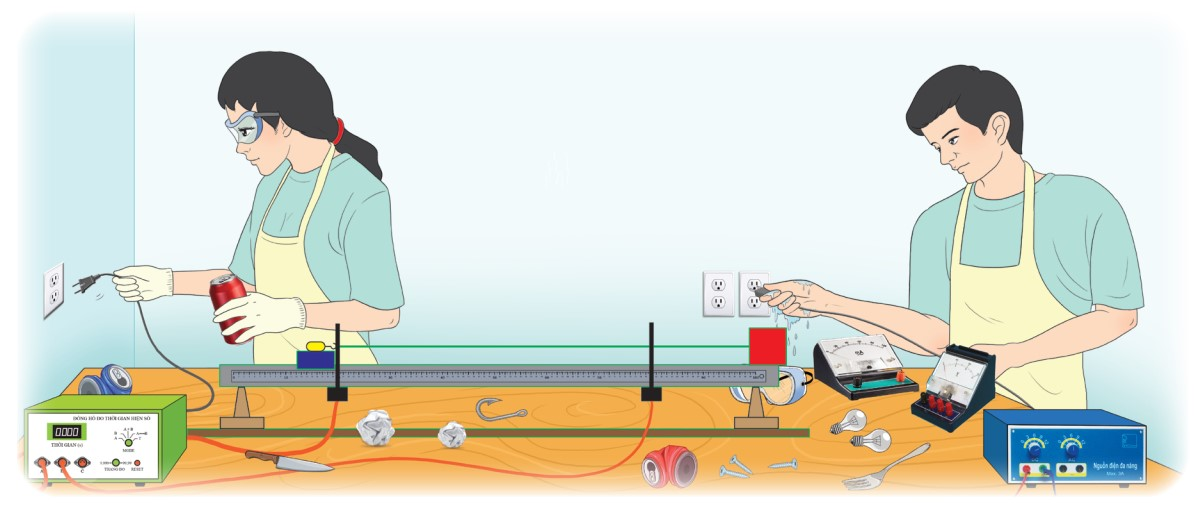
\includegraphics[width=0.8\linewidth]{figs/BAI2-1}}\\
		\multicolumn{2}{|L{17cm}|}{\dotfill}\\
		\multicolumn{2}{|L{17cm}|}{\dotfill}\\
		\multicolumn{2}{|L{17cm}|}{\dotfill}\\
		\multicolumn{2}{|L{17cm}|}{\dotfill}\\
		\hline
	\end{longtable}
\end{center}
Một số biển báo cảnh báo cùng một số trang thiết bị bảo hộ thường gặp.
\begin{center}
	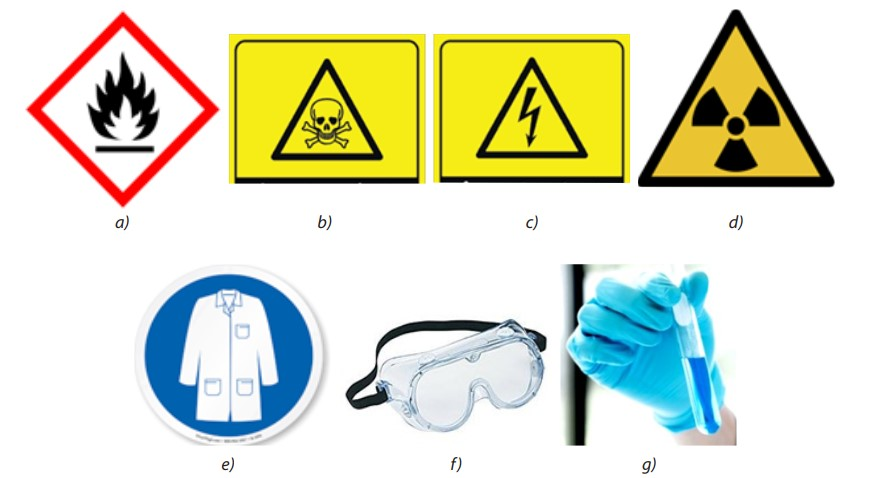
\includegraphics[width=0.8\linewidth]{figs/BAI2-2}
\end{center}